\documentclass{../res/univ-projet}

%Import des packages utilisés pour le document
\usepackage[utf8x]{inputenc}
\usepackage[francais]{babel}
\usepackage[T1]{fontenc}
%\usepackage{array}
%\usepackage{hyperref}
%\usepackage{tabularx, longtable}
%\usepackage[table]{xcolor}
%\usepackage{fancyhdr}
%\usepackage{lastpage}

\definecolor{gris}{rgb}{0.95, 0.95, 0.95}

%Redéfinition des marges
%\addtolength{\hoffset}{-2cm}
%\addtolength{\textwidth}{4cm}
\addtolength{\topmargin}{-1cm}
\addtolength{\textheight}{1cm}
\addtolength{\headsep}{0.8cm} 
\addtolength{\footskip}{-0.2cm}


%Import page de garde et structures pour la gestion de projet
%\usepackage{structures}

%Variables
\logo{../res/logo_univ.png}
\title{Spécification Technique de Besoin}
\author{Kheireddine \bsc{Berkane}, Nasser \bsc{Adjibi}}
\projet{Compilateur LLVM}
\projdesc{Langage jouet Kawa}
\filiere{M1GIL - Conduite de Projet}
\version{0.7}
\relecteur{Pierre-Luc \bsc{BLOT}, Alexandre \bsc{PETRE}}
%\signataire{Florent \bsc{NICART}}
\date{\today}

\histentry{0.1}{04/11/2014}{Version initiale.}
\histentry{0.1.5}{18/11/2014}{Définition des cas d'utilisations et des exigences.}
\histentry{0.2}{03/12/2014}{Modifications par rapport au retour client du 25/11/2014.}
\histentry{0.3}{10/12/2014}{ \begin{itemize}
								 \item Les parties événements déclenchants ont été détaillées.
								 \item Les parties flots d'exceptions, ainsi que les conditions d’arrêts de toutes les exigences fonctionnelles ont été détaillées.
								 \item L'ajout des exigences opérationnelles d'interface.
								 \item Correction des erreurs signalées lors de la réunion client 04/12/2014.	
							 \end{itemize}	 	
								 }
\histentry{0.4}{22/12/2014}{ \begin{itemize}
\item Les parties événements déclenchants ont été modifiées et structurées sous forme d'une liste.
\item Les parties flots d'exceptions, ainsi que les conditions d’arrêts de toutes les exigences fonctionnelles ont été été modifiées et structurées sous forme d'une liste.
\item La suppression des exigences opérationnelles d'interface après une remarque faite par le prof du TP gestion de projet.
\item Changement de priorité de l'exigence fonctionnelle EF\_4 en secondaire car elle dépend de l'exigence EF\_3 qui est secondaire.
\item Correction des erreurs signalées lors du retour client par mail le 19/12/2014.	
\end{itemize}	 	
}
\histentry{0.5}{18/01/2015}{ \begin{itemize}
\item Élimination des exigences de réalisations qui correspondent aux exigences fonctionnelles afin d'éviter les redondances inutiles. 
\item La partie des exigences fonctionnelles a été détaillée ainsi que les scénarios des exceptions ont été spécifiés afin de faciliter les tests après.
\item Modifications apportées par rapport à la revue du lancement du projet 19/01/2015.
\end{itemize}
}
\histentry{0.6}{11/04/2015}{ 
\begin{itemize}
\item Élimination de l'exigence fonctionnelle EF\_3 : Compiler une application en mode partagé 
\item Élimination de l'exigence fonctionnelle EF\_4 : Compiler une bibliothèques partagée
\item Élimination de l'exigence fonctionnelle EF\_6 : Indiquer les chemins des dépendances entre le source de l'application et des modules (classe/interface) externes
\item Élimination de l'exigence de réalisation EXR\_4 : Compilation d'application partagée
\item Élimination de l'exigence de réalisation EXR\_6 : Compilation de bibliothèque partagée
\item Élimination de l'exigence de réalisation EXR\_25 : Définition d'attributs ou de variables de type \textbf{value}
\item Élimination de l'exigence de réalisation EXR\_26 : Définition méthode value
\item Élimination de l'exigence de réalisation EXR\_41 :  Gestion des exceptions
\item Changement du diagramme de cas d'utilisation après la discussion avec client afin de réduire quelques exigences fonctionnelles et de réalisation 
\end{itemize}
}

\newpage
\histentry{0.7}{15/04/2015}{ 
\begin{itemize}
\item Mettre l'exigence fonctionnelle EF\_3 : Afficher la version du compilateur en secondaire
\item Élimination de l'exigence fonctionnelle EF\_4 :Activer l'affichage en couleur
\item Élimination de l'exigence de réalisation EXR\_5 : Garbage collector
\end{itemize}
}


% -- Début du document -- %
\begin{document}

%Page de garde
\maketitle
\newpage
%La table des matières
\tableofcontents
\newpage

\section{Objet}

% Présentation succinte du sujet et hyp de travail.
LLVM est une infrastructure modulaire permettant la réalisation de
chaînes de compilation et conçue pour l'optimisation. Elle met en oeuvre
une représentation intermédiaire du code qui permet de découpler les
langages de l'architecture. Nore objectif est de réaliser, à l'aide de
l'infrastructure LLVM, un comilateur pour un langage jouet, que nous
appellerons Kawa, ce dernier doit supporter:
 \begin{itemize}
 	\item	Les classes, les classes abstraites, les interfaces
	\item   L'héritage
	\item   Le polymorphisme
	\item   Le système de types sera composé des types primitifs
	  (int, float, etc.), des classes et des interfaces
	\item   Les instructions de contrôle telles ques (if/else, for,
	  while/do, switch, etc.).
	\item   Les méthodes seront définies de manière identique à Java
	  execpté que les paramètres pourront être préfixés du mot clé
	  \bsc{value} (transmission par valeur au lieu de référence)
 \end{itemize}


\subsection{Besoins opérationnels}
\subsection{Objectifs techniques}
\subsection{Contraintes et recommendations}
\subsection{Résultats attendus}

\section{Documents applicables et de référence}
% Liste des
% - Références des documents quidefinissent formellement les principes
%   directeurs et le hypothèse de travail prise en compte pour l'établissement de la spécification.
% - Références des documents cités dans la STB au titre d'explication ou de justification.
Différents documents de référence :
\begin{itemize}

\item Le site LLVM \href{http://llvm.org}{llvm.org}.
\item Le document de spécification du client \href{file:../client/spec1.pdf}{Spec1.pdf}
\end{itemize}

\section{Terminologie et sigles utilisés}
  \begin{itemize}
  	\item LLVM : (Low Level Virtual Machine) est une infrastructure de compilateur conçue optimisation à la compilation.
	\item Kawa : langage jouet qui reprend quelques fonctionnalités de java.
	\item Clang : compilateur pour le langage c++, son interface de bas niveau  se base sur des bibliothèques llvm pour la compilation. Il est utilisé par APPELE.
	\item GIT : logiciel qui permet de stocker un ensemble de fichiers en conservant la chronologie de toutes les modifications qui ont été effectuées dessus.
	\item ELF : (Executable and Linkable Format) est un format de fichier binaire utilisé pour l'enregistrement de code compilé (objets, exécutables, bibliothèques de fonctions).
	\item Ubuntu : Distribution linux sur base Debian.
	\item C++ : Langage de programmation orienté objet bas niveau.
	\item POO : Programmation orientée objet.
	\item Makefile : Fichier regroupant des instructions de compilation avec gestion de dépendances.
  \end{itemize}

\section{Exigences fonctionnelles}
\subsection{Présentation de la mission du produit logiciel}

\begin{tabular}{|>{\centering}p{1cm}|>{\centering}p{7cm}|>{\centering}p{2.5cm}|>{\centering}p{3cm}|}
  \hline
  \color{white}\cellcolor{blue}\bfseries{Id}&
  \color{white}\cellcolor{blue}\bfseries{Intitulé}&
  \color{white}\cellcolor{blue}\bfseries{Acteur(s)}&
  \color{white}\cellcolor{blue}\bfseries{Priorité}\\
  \cr
  \hline EF\_1&
  Afficher l'aide&
  Utilisateur&
  Indispensable
  \cr
  \hline EF\_2&
  Compiler une application en mode monolithique &
   Utilisateur&
  Indispensable
  \cr
  \hline EF\_3&
  Compiler une application en mode partagé& 
  Utilisateur&
  Secondaire
  \cr
  \hline EF\_4&
  Chosir un nom pour l'exécutable&
   Utilisateur&
  Important
  \cr
  \hline EF\_5&
  Compiler des bibliothèques&
  Utilisateur&
  Important
  \cr
  \hline EF\_6&
  Afficher la version du compilateur&
  Utilisateur&
  Important
  \cr
  \hline EF\_7&
  Définir des dépendances entre sources et classes&
  Utilisateur&
  Important
  \cr
  \hline EF\_8&
  Activer l'affichage en couleur&
  Utilisateur&
  Important
  \cr
  
  \hline
\end{tabular}\\

\newpage

\begin{figure}
  \centering
  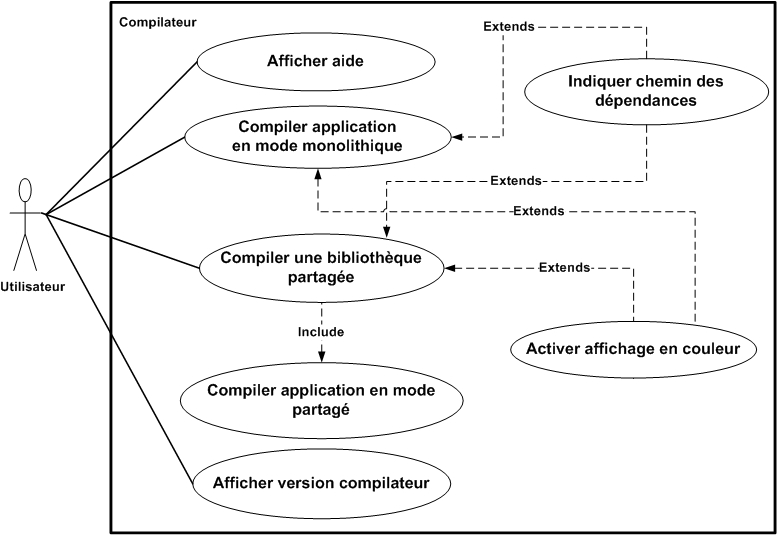
\includegraphics[scale=0.8]{../res/stb/vs_finale_usecase1.jpg}
  \caption{\textbf{Cas d'utilisations du compilateur kawa.}}
\end{figure}

%Cas d'utilisation
\subsection{Cas d'utilisation EF\_1}
\fiche
{Afficher l'aide}                    % Nom du cas d'utilisation
{Utilisateur du compilateur}                               % Acteurs concernés
{                                                % Description
  le compilateur affiche 
   la liste des options du compilateur sur la sortie standard à travers une ligne de commande.
}
{
  L'ordre de priorité entre le commutateur de help (-h ou -\hspace{0.1mm}-help) et le commutateur de version (-v ou -\hspace{0.1mm}-version) est définit par le commutateur en premier paramètre. Le commutateur -h/-\hspace{0.1mm}-help est le premier paramètre obligatoirement.
}                                                % Préconditions
{Commutateur de ligne de commande :kawac -h ou -\hspace{0.1mm}-help }                             % Evénements déclenchants
{L'aide a été affichée correctement et la main est redonnée à l'utilisateur pour entrer d'autres commutateurs.}                       % Conditions d'arrêt
% {0.6}{../res/stb/usecase2_flot_event.png}      % Diagramme
{} % acteur(s)
{} % system
{} % flot exceptionsb
 % fin usecase EF_1

\subsection{Cas d'utilisation EF\_2}
\fiche
{Compiler une application en mode monolithique}                    % Nom du cas d'utilisation
{Utilisateur du compilateur}                               % Acteurs concernés
{                                                % Description
  L'utilisateur introduit un ensemble de modules (classe/interface)
  kawa afin de les précompiler et de générer une application sous forme d'un seul exécutable.
}
{
	Afin de permettre la compilation dans ce mode monolithique il faut:
	\begin{itemize}
  	\item Indiquer l’emplacement des fichiers sources de l'application.
  	\item Introduire le commutateur  \textbf {-m}  en premier paramètre dans la ligne de commande permettant la compilation.
  	\item L'absence des deux commutateurs (-h ou -\hspace{0.1mm}-help) et (-v ou -\hspace{0.1mm}-version) en premier paramètre.
  	\end {itemize}
}                                                % Préconditions
{

Afin de pouvoir lancer la compilation dans ce mode l'utilisateur  doit: 
\begin{itemize}
  	\item Indiquer au moins un module (une classe avec une méthode main qui constitue le point d'entrée d'une application).
  	\item Introduire une ligne de commande avec un commutateur d'action: kawac -m filessources.
 \end {itemize}

}    % Evénements déclenchants
{
	\begin{itemize}
  	\item La compilation s'est terminée sans erreurs dans ces différentes étapes d’analyses.
  	\item La production d’un unique fichier exécutable sous le format d'ELF  qui ne dépend d'aucune bibliothèque kawa ainsi que le nom du fichier exécutable correspond au nom du module contenant la méthode main.
\end {itemize}
  
}  % Conditions d'arrêt
%{0.6}{../res/stb/usecase2_flot_event.png} 		 % Diagramme
{                                                % Flots d'exceptions
  
}
{} % system
{
La compilation peut être interrompue pour divers raisons, on cite:

	\begin{itemize}
  	\item \textbf {EF\_2\_EXC\_1}: Le fichier de sortie n'a pu être créé.
  	\item  \textbf {EF\_2\_EXC\_2}: Le code source d'un des modules de l'application comporte une erreur syntaxique, l'erreur rencontrée pendant cette étape d'analyse est renvoyée sur la sortie standard du compilateur.
  	\item \textbf {EF\_2\_EXC\_3}: Le code source d'un des modules (classe/interface) dont dépend le programme est introuvable. Un message renvoyé par le compilateur indique le nom du (ou des) module(s) manquants sur la sortie standard.
  	\item \textbf {EF\_2\_EXC\_4}: Le code source d'un des modules de l'application comporte une erreur sémantique, exemple : l'incompatibilité de type statique lors d'une opération d'affectation.
  	\item \textbf {EF\_2\_EXC\_5}: Aucun des modules indiqués ne comporte le point d'entrée (main).
  	\item \textbf {EF\_2\_EXC\_6}: Plusieurs méthodes main ont été trouvées parmi les classes indiquées dans le source, le compilateur renvoie la liste des points d'entrée trouvés sur la sortie standard.
  	\end {itemize}
 } % flot exceptions
% Fin de la fiche du cas d'utilisation 1.


%Cas d'utilisation 2
\subsection{Cas d'utilisation EF\_3}
\fiche
{Compiler une application en mode partagé}                    % Nom du cas d'utilisation
{Utilisateur du compilateur}                               % Acteurs concernés
{                                                % Description
  L’utilisateur introduit un ensemble de sources kawa
 qui peuvent appeler des bibliothèques externes. Le compilateur doit être capable de trouver les bibliothèques pour les utiliser ou bien  de les recompiler si nécessaire. La différence entre ce mode et le mode monolithique est que le fichier exécutable et la bibliothèque sont indépendants avant le lancement de l’application, et peuvent être maintenus séparément à l'encontre du mode monolithique qui génère un seul exécutable regroupant le tout. Pour les bibliothèques partagées l'édition des liens se fait à l’exécution (au moment du lancement du programme) au contraire des bibliothèques statiques où l'édition des liens se fait dans la phase de compilation. 
}
{
	Afin de permettre la compilation dans ce mode il faut:
	\begin{itemize}
  	\item Spécifier l’emplacement des fichiers sources de l'application.
  	\item L'absence du commutateur  \textbf {-m}  en premier paramètre.
  	\item L'absence des deux commutateurs (-h ou -\hspace{0.1mm}-help) et (-v ou -\hspace{0.1mm}-version) en premier paramètre.
  	\end {itemize}

	
}                                                % Préconditions
{

Afin de pouvoir lancer la compilation dans ce mode l'utilisateur  doit: 
\begin{itemize}
  	\item Indiquer au moins un module (une classe avec une méthode main qui constitue le point d'entrée d'une application).
  	\item Introduire une ligne de commande sans commutateur d'action (fonctionnement par défaut): kawac filessources [options].
 \end {itemize}
 L'utilisateur peut éventuellement compiler des fichiers des modules qui ne sont pas forcément en relation avec l'application à compiler.
}  % Evénements déclenchants
{
\begin{itemize}
  	\item La compilation s'est terminée sans erreurs dans ces différentes étapes d’analyses.
  	\item La production d’un unique fichier exécutable sous le format d'ELF et qui n'est pas sous l'extension (.so), le nom du fichier exécutable correspond au nom du module contenant la méthode main.
\end {itemize}
  	} % Conditions d'arrêt
%{0.6}{../res/stb/usecase2_flot_event.png} 		 % Diagramme
{                                                % Flots d'exceptions
  
}{} % system
{La compilation peut être interrompue pour divers raisons, on cite:

\begin{itemize}
  	\item \textbf {EF\_3\_EXC\_1}: Le fichier de sortie n'a pu être créé.
  	\item  \textbf {EF\_3\_EXC\_2}: Le code source d'un des modules de l'application comporte une erreur syntaxique, l'erreur rencontrée pendant cette étape d'analyse est renvoyée sur la sortie standard du compilateur.
  	\item \textbf {EF\_3\_EXC\_3}: Un module (classe ou interface) de l'application fait référence à un symbole externe introuvable, soit le paquetage externe contenant le symbole n'existe pas, ou bien il n'a pu être compiler à cause d'une erreur.
  	\item \textbf {EF\_3\_EXC\_4}: Le code source d'un des modules de l'application comporte une erreur sémantique, exemple : l'incompatibilité de type statique lors d'une opération d'affectation.
  	\item \textbf {EF\_3\_EXC\_5}: Aucun des modules indiqués ne comporte le point d'entrée (main).
  	\end {itemize}
 } % flot exceptions
% Fin de la fiche du cas d'utilisation 2.


%Cas d'utilisation
\subsection{Cas d'utilisation EF\_4}
\fiche
{Compiler une bibliothèques partagée}                      % Nom du cas d'utilisation
{Utilisateur du compilateur}                               % Acteurs concernés
{                                                % Description
    L'utilisateur peut compiler des bibliothèques partagée en introduisant le nom du paquetage contenant les sources de la bibliothèque, la bibliothèque elle même peut contenir des sous bibliothèques (sous paquetages), pour notre cas d'étude chaque sous paquetages aura son propre fichier (.so).

     Le compilateur produit du code compilé destiné à être partagé entre plusieurs différents programmes, l'extension de la bibliothèque produite sera (.so => Shared Object) qui est un unique fichier exécutable pour tout le paquetage. On ne peut compiler une bibliothèque partagée que dans un mode partagé avec la non présence cette fois ci de la méthode main.      
}
{
	Afin de permettre la compilation d'une bibliothèque partagée expicitement il faut:
	\begin{itemize}
  	\item Indiquer le nom du répertoire contenant les fichiers sources de la bibliothèque.
  	\item L'absence du commutateur \textbf {-m} en premier paramètre, pour indiquer qu'on est dans un mode paratgé.
  	\item L'absence des deux commutateurs (-h ou -\hspace{0.1mm}-help) et (-v ou -\hspace{0.1mm}-version) en premier paramètre.
  	\end {itemize}
}               % Préconditions
{
	Afin de pouvoir lancer la compilation de la bibliothèque l'utilisateur doit:
	\begin{itemize}
  	\item Indiquer le nom du paquetage contenant les sources de la bibliothèque.
  	\item Introduire la ligne de commande sans les commutateurs d'actions: kawac filessources [options].
  	\end {itemize}

} % Evénements déclenchants
{{                                                % Flots d'exceptions
  
}{}
La compilation s'est terminée sans erreurs dans ces différentes étapes d'analyses et a comme résultats:
	\begin{itemize}
  	\item La production d'une bibliothèque dynamique dont le nom et l'emplacement correspondent à ceux du paquetage indiqué par l'utilisateur.
  	\item La bibliothèque va contenir les symboles de liaison pour tous les éléments publiques du paquetage.
  	\end {itemize}

} % Conditions d'arrêt
%{0.6}{../res/stb/usecase3_flot_event.png}     % Diagramme
{                                                % Flots d'exceptions
 
}{} % system
{	La compilation peut être interrompue pour divers raisons, on cite:
	\begin{itemize}
  	\item \textbf {EF\_4\_EXC\_1}: Le répertoire du paquetage est vide.
  	\item \textbf {EF\_4\_EXC\_2}: Erreur rencontrée lors de l'analyse syntaxique de l'un des modules du paquetage.
  	\item \textbf {EF\_4\_EXC\_3}: Erreur rencontrée lors de l'analyse sémantique de l'un des modules du paquetage.
  	\item \textbf {EF\_4\_EXC\_4}: Un module (classe ou interface) de la bibliothèque fait référence à un symbole externe introuvable, soit le paquetage externe contenant le symbole n'existe pas, ou bien il n'a pu être compiler à cause d'une erreur.

  	\item \textbf {EF\_4\_EXC\_5}: Un point d'entrée (main) a été trouvé dans l'un des modules du paquetage.
  	\end {itemize}

} % flot exceptions
% Fin de la fiche du cas d'utilisation 3.
%Cas d'utilisation
\subsection{Cas d'utilisation EF\_5}
\fiche
{Afficher la version du compilateur}                      % Nom du cas d'utilisation
{Utilisateur du compilateur}                               % Acteurs concernés
{                                                % Description
   
L'utilisateur peut savoir la version du compilateur avec le quel compile ses sources et ses bibliothèques  à travers un commutateur de ligne de commande.   
}
{
   L'odre de priorité entre le commutateur de help (-h ou -\hspace{0.1mm}-help) et le commutateur de version (-v ou -\hspace{0.1mm}-version) est définit par la première occurrence de l'un des deux commutateur i-e si nous avons un \textbf {-v} avant un \textbf {-h}, le compilateur annule tout le reste et affiche la version
}                                                % Préconditions
{Commutateur de ligne de commande:kawac -v ou -\hspace{0.1mm}-version}                             % Evénements déclenchants
{La version est affichée sur la sortie standard du compilateur.}                       % Conditions d'arrêt
%{0.6}{../res/stb/usecase3_flot_event.png}     % Diagramme
{                                                % Flots d'exceptions
 
}{} % system
{} % flot exceptions
% Fin de la fiche du cas d'utilisation 3.
%Cas d'utilisation
\subsection{Cas d'utilisation EF\_6}
\fiche
{Indiquer les chemins des dépendances}          % Nom du cas d'utilisation
{Utilisateur du compilateur}                               % Acteurs concernés
{                                                % Description
	Afin de permettre la définition  des schémas de dépendances entre le source de l'application et des modules externes (peuvent être des bibliothèques déjà compilées) il faut:   
	\begin{itemize}
  	\item Spécifier le chemin vers le(s) module(s) externe(s).
  	\item L'absence du commutateur  \textbf {-m}  en premier paramètre, car on est obligatoirement dans un mode de compilation en partagé
  	\item L'absence des deux commutateurs (-h ou -\hspace{0.1mm}-help) et (-v ou -\hspace{0.1mm}-version) en premier paramètre.
  	\end {itemize}
}
{
  
}                                                % Préconditions
{ 
	Afin de pouvoir lancer la compilation avec les différentes dépendances en interne:
	\begin{itemize}
  	\item L'utilisateur introduit des schémas de dépendances grâce au commutateur: kawac filessources -d path.
  	\item L'utilisateur indique les sources de son appelication.
  	\end {itemize}

}                             % Evénements déclenchants
{Fin de la compilation sans erreurs dans ces différentes étapes d'analyses, ainsi que la reconnaissance de tous les schémas de dépendances introduit par l'utilisateur.}                       % Conditions d'arrêt
%{0.6}{../res/stb/usecase3_flot_event.png}     % Diagramme
{                                                % Flots d'exceptions
 
}{} % condition d'arret
{
La compilation peut être interrompue pour divers raisons, on cite:
	\begin{itemize}
  	\item \textbf {EF\_6\_EXC\_1}: Le module indiqué dans le chemin de dépendance est introuvable.
  	\item \textbf {EF\_6\_EXC\_2}: Erreur rencontrée lors de l'analyse syntaxique de l'un des modules du code source.
  	\item \textbf {EF\_6\_EXC\_3}: Erreur rencontrée lors de l'analyse sémantique de l'un des modules du du code source.
  	\item \textbf {EF\_6\_EXC\_4}: Le source contenant le point d'entrée est introuvable, un message d'erreur est renvoyé par le compilateur sur la sortie standard.
  	\end {itemize}
} % flot exceptions
% Fin de la fiche du cas d'utilisation 3.

%Cas d'utilisation
\subsection{Cas d'utilisation EF\_7}
\fiche
{Activer l'affichage en couleur}          % Nom du cas d'utilisation
{Utilisateur du compilateur}                               % Acteurs concernés
{                                                % Description
   
  L'utilisateur peut activer l'option de l'affichage en couleur, afin de décorer les messages renvoyés par le compilateur la sortie standard dans les différents modes de compilation.   
}
{
  
}                                                % Préconditions
{Commutateur de ligne de commande:kawac filessource -\hspace{0.1mm}-color}  % Evénements déclenchants (--help) \verb+kawac -h ou --help+ -----> pour creer u espace entre --
{Le code présent sur la sortie standard a été colorié.}                       % Conditions d'arrêt
%{0.6}{../res/stb/usecase3_flot_event.png}     % Diagramme
{                                                % Flots d'exceptions
 
}{} % system
{} % flot exceptions
% Fin de la fiche du cas d'utilisation 3.

\newpage
\section{Exigences opérationnelles}
Pas de spécifications concernant cette section.

\begin{tabular}{|>{\centering}p{1,5cm}|>{\centering}p{10cm}|>{\centering}p{3cm}|}
  \hline
  \color{white}\cellcolor{blue}\bfseries{Id}&
  \color{white}\cellcolor{blue}\bfseries{Intitulé}&
  \color{white}\cellcolor{blue}\bfseries{Priorité}\\
  \cr
  \hline
\end{tabular}\\

\section{Exigences opérationnelles d'interface}
Pas de spécifications concernant cette section.

\begin{tabular}{|>{\centering}p{1,5cm}|>{\centering}p{10cm}|>{\centering}p{3cm}|}
  \hline
  \color{white}\cellcolor{blue}\bfseries{Id}&
  \color{white}\cellcolor{blue}\bfseries{Intitulé}&
  \color{white}\cellcolor{blue}\bfseries{Priorité}\\
  \cr
  \hline
\end{tabular}\\


\section{Exigences de qualité}

\begin{tabular}{|>{\centering}p{1,5cm}|>{\centering}p{10cm}|>{\centering}p{3cm}|}
  \hline
  \color{white}\cellcolor{blue}\bfseries{Id}&
  \color{white}\cellcolor{blue}\bfseries{Intitulé}&
  \color{white}\cellcolor{blue}\bfseries{Priorité}\\
  \cr
  \hline
  EQ\_1&
  les messages d’erreurs
renvoyés par le compilateur doivent être explicites, les plus fines possibles et
surtout par rapport à ce qu'il s'est passé.&
  Important
  \cr
  \hline
\end{tabular}\\

\section{Exigences de réalisation}
  \begin{tabular}{|>{\centering}p{1,5cm}|>{}p{10cm}|>{\centering}p{3cm}|}
  \hline
  \color{white}\cellcolor{blue}\bfseries{Id}&
  \color{white}\cellcolor{blue}\bfseries{Intitulé et Description}&
  \color{white}\cellcolor{blue}\bfseries{Priorité}\\

  \cr
  \hline
  EXR\_1&
  {\bfseries Nommage des fichiers de sortie} : On pourra choisir le nom du fichier à l'issue de la compilation.&
  Indispensable
  \cr
  \hline
  EXR\_2&
  {\bfseries Reconnaissance de la grammaire KAWA} : KAWAC est capable de dire si le code est valide pour la grammaire de KAWA, et émettre des erreurs pour signaler à quelle position dans le texte, et si possible proposer une solution au problème.&
  Indispensable
  \cr
  \hline
  EXR\_3&
  {\bfseries Compilation d'application en monolithique} : KAWAC pourra compiler des fichiers et fournir un exécutable qui n'a pas besoin de bibliothèques externes pour fonctionner. L'ensemble du code donné en entrée devra fournir une méthode main, qui sera le point d'entrée de l'application.&
  Indispensable
  \cr
  \hline
  EXR\_4&
  {\bfseries Compilation d'application partagée} : KAWAC pourra compiler des fichiers et fournir un exécutable. L'exécutable s'il le faut dépendra de ressources externes pour pouvoir fonctionner. Le code en entrée devra fournir une méthode main, qui sera le point d'entrée de l'application.&
  Important
  \cr
  \hline
  EXR\_5&
  {\bfseries Compilation de bibliothèque partagée} : KAWAC pourra compiler des fichiers et fournir une nouvelle bibliothèque. La bibliothèque s'il le faut dépendra de ressources externes pour pouvoir fonctionner. Le code en entrée devra ne pas contenir de methode main.&
  Important

  \cr
  \hline
  EXR\_6&
  {\bfseries Gestion des mots clés} : KAWA spécifie dans sa grammaire une liste de mots réservés. Ces mots sont utilisés par le développeur pour des actions prédéfinies, et ne peuvent être utilisés comme nom de méthodes, d'attributs ou de variables.&
  Indispensable

  \cr
  \hline
  EXR\_7&
  {\bfseries Fichier de sortie au format ELF} : Le compilateur utilisera le format ELF pour la production des fichiers en sortie. Les fichiers contiendront une section contenant les information permettant la résolution des liens d’appel de fonctions. Les fichiers exécutables utiliseront ces informations pour monter en mémoire les références des bibliothèques externes lors de la phase d'édition des liens.&
  Indispensable

  \cr
  \hline
  EXR\_8&
  {\bfseries Gestion de la mémoire} : La gestion de la mémoire est automatisée. Les réservations et libérations des espaces mémoires utilisés par les objets s’effectuent sans une intervention directe du développeur. Les objets non référencés sont susceptibles d'être désalloués. Une demande d'allocation mémoire ne peut être est faite par l'utilisateur que grâce au mot clé  \textbf{new} permettant d'instancier un objet.&
  Important

  \cr
  \hline
  EXR\_9&
  {\bfseries Importation de packages} : Le développeur peut utiliser des entités présents dans des packages externes, grâce au mot clé \textbf{import}.&
  Important

  \cr
  \hline  
  EXR\_10&
  {\bfseries Déclaration de package} : Le développeur déclarer un package grâce au mot clé \textbf{package}.&
  Indispensable

  \cr
  \hline

\end{tabular}\\

\newpage
\begin{tabular}{|>{\centering}p{1,5cm}|>{}p{10cm}|>{\centering}p{3cm}|}

  \hline
  EXR\_11&
  {\bfseries Reconnaissance et compilation de classes} : KAWAC est capable de reconnaître et compiler des classes écrites en KAWA. La déclaration d'une classe se fait grâce au mot clé \textbf{class}. Une classe est déclarée dans un fichier \textbf{.kawa}, et rend en sortie un fichier \textbf{.klass}. Une classe permet de définir des attributs, des constructeurs et des méthodes. Elle peut être instanciée et utilisée par une ou plusieurs applications. Une classe peut dériver une classe abstraite ou une autre classe et implémenter plusieurs interfaces(Veuillez consulter la grammaire KAWA en annexe pour la syntaxe).&
  Indispensable

  \cr
  \hline

  EXR\_12&
  {\bfseries Reconnaissance et compilation de classes abstraites} : KAWAC est capable de reconnaître et compiler des classes abstraites écrites en KAWA.La déclaration d'une classe abstraite se fait grâce aux mots clés abstract class. Une classe abstraite est déclarée dans un fichier \textbf{.kawa}, et rend en sortie un fichier \textbf{.klass}. Contrairement à une classe normale, une classe abstraite ne peut être instanciée. Elle est faite pour être dériver par une autre classe. Cependant, en plus des fonctionnalités d'une classe normale, une classe abstraite peut définir des prototypes de méthodes qui devront être implémentées par les classes filles de la classe abstraite.(Veuillez consulter la grammaire KAWA en annexe pour la syntaxe).&
  Indispensable

  \cr
  \hline

\hline
  EXR\_13&
  {\bfseries Reconnaissance et compilation d'interfaces} : KAWAC est capable de reconnaître et compiler des interfaces écrites en KAWA. La déclaration d'une interface se fait grâce au mot clé \textbf{interface}. Une interface est déclarée dans un fichier \textbf{.kawa}, et rends en sortie un fichier \textbf{.klass}. Une interface ne peut que déclarer les prototypes des méthodes que devront implémenter les classes qui implémenteront l’interface. Ces dernières ne peuvent être que de portée publique et sont abstraites. Une interface ne contient ni attribut, ni constructeur. Une interface est destinée à être implémentée par une classe ou partiellement par une classe abstraite. Le développeur utilisera le mot clé \textbf{extends} pour spécifier l’implémentation d'une ou plusieurs interfaces(Veuillez consulter la grammaire KAWA en annexe pour la syntaxe).&
  Indispensable

  \cr
  \hline
  EXR\_14&
  {\bfseries Prise en charge du polymorphisme ad-hoc}: Si plusieurs méthodes portent le même nom, KAWA est capable de déterminer la méthode à appeler lors de l'exécution de l'application en fonction de la signature de la méthode.&
  Important

  \cr
  \hline
  EXR\_15&
  {\bfseries Prise en charge du polymorphisme de sous-type} : KAWA est capable de déterminer lors de l'exécution la méthode en fonction du type dynamique de la classe appelante. KAWAC n'autorise pas le cast d'objets.&
  Important

  \cr
  \hline
  EXR\_16&
  {\bfseries Dérivation d'entités} : En utilisant le mot clé \textbf{extends} dans la déclaration d'une classe, d'une classe abstraite ou d'une interface, l'utilisateur est capable de dériver ou d’implémenter une classe ou des interfaces. Une classe peut dériver une autre classe ou une classe abstraite. Si non abstraite dérive une classe abstraite ou une interface, elle doit implémenter toutes les méthodes abstraites de la classe qu'elle dérive. Une classe ne peut dériver qu'une classe à la fois, mais peut implémenter plusieurs interfaces. Une interface peut dériver plusieurs interfaces, mais ne peut dériver une classe.&
  Important

  \cr
  \hline

\end{tabular}\\
\newpage
\begin{tabular}{|>{\centering}p{1,5cm}|>{}p{10cm}|>{\centering}p{3cm}|}

  \hline

  EXR\_17&
  {\bfseries Mécanisme de constructeur} : Chaque classe, pour être instancié, fournit une ou plusieurs méthodes qui permettront son instanciation.
  KAWAC fournira un constructeur si aucun constructeur n'est pas définit. L'instanciation se fait grâce au mot clé \textbf{new}, et retourne une référence vers un espace mémoire stockant l'objet. Une classe abstraite peut définir un constructeur, mais ne peut instancier. Une interface n'a pas de constructeur.(Veuillez consulter la grammaire KAWA en annexe pour la syntaxe).&
  Indispensable
  \cr
  \hline


  EXR\_18&
  {\bfseries Mécanisme de finalisation} : Chaque objet fournit une méthode qui sera appelée lors de sa destruction par le garbage collector. Si aucune méthode n'est définie par le développeur, KAWAC en fournira une par défaut.&
  Secondaire

  \cr
  \hline
  EXR\_19&
  {\bfseries Reconnaissance et définition de méthode et de variables} : On peut déclarer un bloc d'instructions paramétrable s'exécutant s'il est appelé.On peut définir des variables temporaires et dont la portée sera limitée au bloc dans lequel elles ont été déclarées. Les variables locales ne sont pas des attributs et ne sont plus accessibles à la fin du bloc d'instruction les déclarant.&
  Indispensable

  \cr
  \hline
  EXR\_20&
  {\bfseries Reconnaissance et définition d'attribut d'objet} : On peut déclarer des champs propres à chaque objet. Les espaces attribués à chaque attribut ne sont accessibles que durant la période de vie de l'objet, par les membres de l'objet ou par un programme externe si l'attribut est déclaré public.&
  Indispensable

  \cr
  \hline
  EXR\_21&
  {\bfseries Définition d'attributs statiques} : On peut définir des espaces mémoires associés aux classes. Les objets instanciant ou dérivant la classe où a été déclaré l'attribut et si la visibilité le permet, pointeront vers la même adresse pour cet attribut. Une méthode statique ne peut accéder aux attributs ou méthodes qui ne sont pas statiques.&
  Important

  \cr
  \hline

  EXR\_22&
  {\bfseries Définition d'attribut de constantes} :Un attribut constant ne peut être modifié après affectation. Il doit avoir été initialisé d'être utilisable par une autre opération que l'affectation.&
  Secondaire

  \cr
  \hline
  EXR\_23&
  {\bfseries Définition d'attributs, de variables ou de méthodes de type value} : En définissant un attribut avec le mot clé \textbf{value}, on aura accès non pas a une référence vers un espace mémoire stockant les données, mais directement a un bloc de données. Dans le cas d'une méthode, la méthode renvoie un bloc de données représentant le résultat.&
  Important

  \cr
  \hline
  EXR\_24&
  {\bfseries Définition méthode a référence} : La méthode renvoie une référence vers un espace mémoire contenant les données de l'objet renvoyé.&
  Indispensable

  \cr
  \hline
  EXR\_25&
  {\bfseries Définition méthode a sans référence} : La méthode ne retourne rien.&
  Indispensable

  \cr
  \hline
  EXR\_26&
  {\bfseries Définition méthode finale} : La méthode ne peut être surchargée ou redéfinie.&
  Secondaire

  \cr
  \hline
  EXR\_27&
  {\bfseries Définition méthode statique} : La méthode peut être accessible à partir du nom de la classe. Une méthode statique ne peut faire appel aux attributs non statiques de sa classe.&
  Important

  \cr
  \hline
  EXR\_28&
  {\bfseries Héritage de méthode} : Une classe dérivant une autre copiera toute les méthodes déjà définit dans l'arborescence de ses ancêtres. Mais ne pourra y accéder que si la visibilité le permet.&
  Indispensable

  \cr 
  \hline

\end{tabular}\\

\newpage
\begin{tabular}{|>{\centering}p{1,5cm}|>{}p{10cm}|>{\centering}p{3cm}|}

  \hline
  EXR\_29&
  {\bfseries Héritage d'attribut} : Une classe dérivant une autre copiera tout les attributs déjà définit dans l’arborescence de ses ancêtres si la visibilité le permet.
  On ne peut pas redéfinir un attribut déjà définit dans la classe ou interface dérivée.&
  Indispensable

  \cr
  \hline
  EXR\_30&
  {\bfseries Redéfinition de méthode} : Une méthode peut être définie avec le nom d'une autre existence, en renvoyant le même type de valeur, ainsi que les mêmes paramétrés dans une autre de l'arborescence de la classe ayant premièrement définit.&
  Important

  \cr
  \hline
  EXR\_31&
  {\bfseries Surcharge des méthode} : Une méthode peut être définie avec le nom d'une autre existence, en renvoyant le même type de valeur, mais avec des paramètres différents.&
  Important

  \cr
  \hline
  EXR\_32&
  {\bfseries Concepte de visibilité :} A l'aide des mots clés, on peut définir la visibilité des attributs et méthodes des classes sur plusieurs niveaux. Privée, pour empêcher l'accès en dehors de la classe. Protégée, pour empêcher l'accès en dehors de la classe, sauf pour les hérités de la classe ou de l'interface. Publique pour autoriser l'accès à tous.&
  Important

  \cr
  \hline
  EXR\_33&
  {\bfseries Portée de variable} : Une variable n'est effective qu'à l’intérieur du bloc à dans lequel elle a été déclarée. &
  Indispensable

  \cr
  \hline

  EXR\_34&
  {\bfseries Gestion des exceptions} : On est capable de provoquer volontairement ou non, une execption qui se propagera dans le programme, jusqu'a ce qu'elle soit rattrapée et traitée par le programme. Si une exception n'est pas traité, l'application devra s'arreter et afficher un message d'erreur sur la sortie des erreurs.&
  Secondaire

  \cr
  \hline

  EXR\_35&
  {\bfseries Reconnaissance des expression conditionnelles} : KAWA admet des expressions conditionnelles. Le programme exécute un bloc d'instruction donné ou un autre selon des condition définies par le développeur.&
  Imporant

  \cr
  \hline
  EXR\_36&
  {\bfseries Reconnaissance des expression de bouclages} : KAWA admet des expressions de bouclage. Le programme répétera l'exécution d'un bloc d’instruction donné tant qu'une condition définies par le développeur est correcte .&
  Important

  \cr
  \hline
  EXR\_37&
  {\bfseries Bloc de classe} : La définition du corps de l'objet se fera a l’intérieur d'un bloc délimité par \{ et \}. Le bloc de classe est le bloc générale contenant toutes les déclarations liées à une classe. A part les importations de packages, la déclaration de l'entête de la classe ou interface ou les commentaires, aucun autre élément ne doit être présent dans le fichier. On ne peut définir qu'une classe par fichier et KAWA n'autorise pas la déclaration de classe imbriquée.&
  Indispensable

  \cr
  \hline
  EXR\_38&
  {\bfseries Bloc d'instruction} : On peut définir une suite d'instructions délimité par \{ et \}. Un bloc d'instruction peut contenir d'autres blocs.&
  Indispensable

  \cr
  \hline
  EXR\_39&
  {\bfseries Reconnaissance des commentaires} : Le développeur peut laisser des commentaires dans le code KAWA. Ces commentaire seront reconnus et ignorés par KAWAC lors de la compilation.&
  Important

  \cr
  \hline

\end{tabular}\\


\end{document}

